\graphicspath{{appendices/imgs/}}
\chapter{Statystyki opisowe pytań kwestionariuszy}\label{appendix:B}

\begin{table}[h!]
    \begin{center}
        \begin{tabular}{|m{12em}|r|r|r|}
            \hline
            Pytanie                                                           & Średnia ocena & Mediana & Odchylenie st. \\
            \hline
            1. Tracę poczucie czasu                                           & 3             & 3       & 1,24           \\
            2. Byłem/-am \newline zainteresowany/-a fabułą gry                & 3,14          & 3       & 1,29           \\
            3. Czuję się inaczej                                              & 2,57          & 2,5     & 1,45           \\
            4. Czułem/-am, że mogę odkrywać różne rzeczy                      & 1,86          & 1,5     & 1,17           \\
            5. Gra wydaje się prawdziwa                                       & 2,14          & 2       & 1,23           \\
            6. Byłem/-am \newline w pełni zajęty/-a grą                       & 3             & 3,5     & 1,52           \\
            7. Denerwuję się                                                  & 2,43          & 2       & 1,28           \\
            8. Czas jakby stanął w miejscu lub się zatrzymał                  & 2,21          & 2       & 1,31           \\
            9. Czuję się \newline rozkojarzony/-a                             & 2,43          & 2       & 1,34           \\
            10. Byłem/-am głęboko \newline skoncentrowany/-a \newline na grze & 2,93          & 3       & 1,38           \\
            11. Zmęczyłem/-am się                                             & 3,29          & 3,5     & 1,54           \\
            12. Granie wydaje się automatyczne                                & 3,29          & 3       & 1,27           \\
            13. Moje myśli \newline biegną szybko                             & 3             & 3       & 1,30           \\
            14. Podobało mi się                                               & 3,36          & 4       & 1,34           \\
            15. Gram bez zastanawiania się jak grać                           & 3,71          & 4       & 1,44           \\
            16. Granie sprawia, \newline że czuję się spokojny/-a             & 3             & 3       & 1,24           \\
            17. Gram dłużej \newline niż zamierzałem/-am                      & 2,64          & 2       & 1,50           \\
            18. Naprawdę wczuwam się w grę                                    & 3,07          & 3       & 1,33           \\
            19. Czuję, że nie mogę przestać grać                              & 2,21          & 2       & 1,48           \\
            \hline
        \end{tabular}
    \end{center}
    \caption{Statystyki opisowe pytań kwestionariusza dla wersji bez AI formularza A}\label{tab1:appendixB_6}
\end{table}

\begin{figure}[h!]
    \centering
    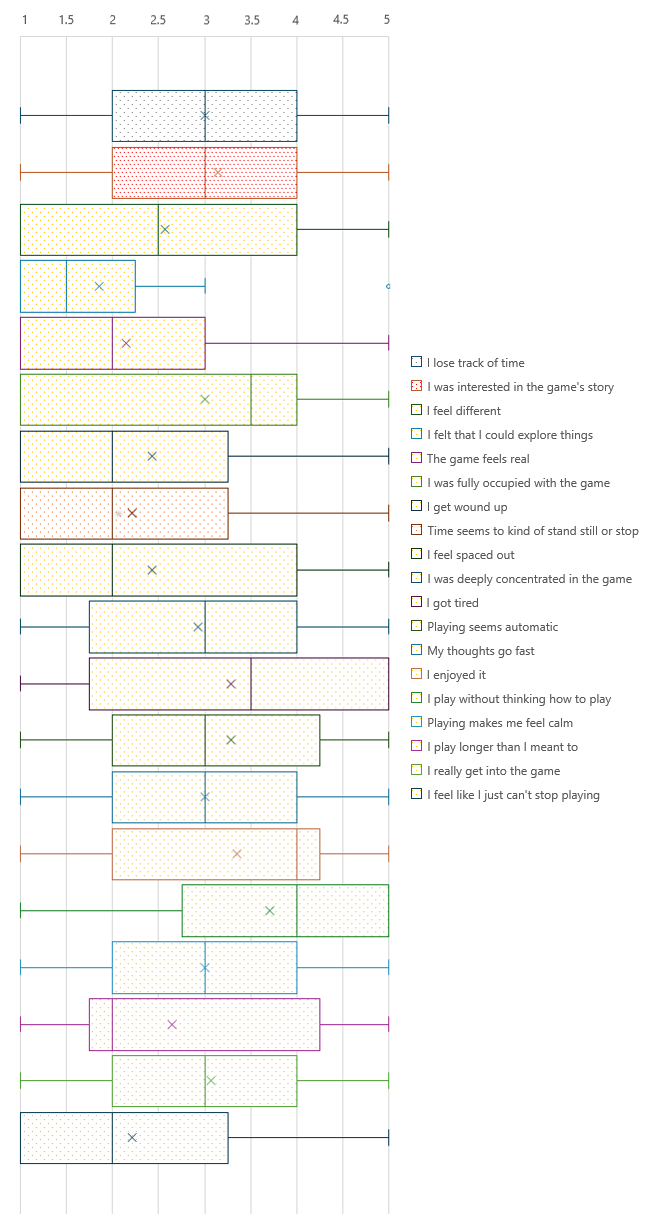
\includegraphics[width=0.8\textwidth]{formA1.png}
    \caption{Wykresy pudełkowe pytań kwestionariusza dla wersji bez AI formularza A}
    \label{fig:appendixB_formA1}
\end{figure}

\begin{table}[h!]
    \begin{center}
        \begin{tabular}{|m{10em}|r|r|r|}
            \hline
            Pytanie                                                           & Średnia ocena & Mediana & Odchylenie st. \\
            \hline
            1. Tracę poczucie czasu                                           & 2,64          & 3       & 1,34           \\
            2. Byłem/-am \newline zainteresowany/-a fabułą gry                & 3,07          & 3,5     & 1,44           \\
            3. Czuję się inaczej                                              & 2,86          & 3       & 1,46           \\
            4. Czułem/-am, że mogę odkrywać różne rzeczy                      & 3,79          & 4       & 1,37           \\
            5. Gra wydaje się prawdziwa                                       & 3             & 3       & 1,41           \\
            6. Byłem/-am \newline w pełni zajęty/-a grą                       & 2,93          & 3       & 1,49           \\
            7. Denerwuję się                                                  & 2,64          & 2       & 1,6            \\
            8. Czas jakby stanął w miejscu lub się zatrzymał                  & 2,36          & 2       & 1,45           \\
            9. Czuję się \newline rozkojarzony/-a                             & 2,29          & 2       & 1,38           \\
            10. Byłem/-am głęboko \newline skoncentrowany/-a \newline na grze & 3             & 3,5     & 1,62           \\
            11. Zmęczyłem/-am się                                             & 3,5           & 4       & 1,22           \\
            12. Granie wydaje się automatyczne                                & 2,29          & 2       & 1,14           \\
            13. Moje myśli \newline biegną szybko                             & 2,64          & 2       & 1,34           \\
            14. Podobało mi się                                               & 3,29          & 4       & 1,44           \\
            15. Gram bez zastanawiania się jak grać                           & 2,93          & 3       & 1,49           \\
            16. Granie sprawia, \newline że czuję się spokojny/-a             & 2,79          & 2       & 1,25           \\
            17. Gram dłużej \newline niż zamierzałem/-am                      & 2,71          & 2       & 1,49           \\
            18. Naprawdę wczuwam się w grę                                    & 3,07          & 3,5     & 1,38           \\
            19. Czuję, że nie mogę przestać grać                              & 2,14          & 2       & 1,46           \\
            \hline
        \end{tabular}
    \end{center}
    \caption{Statystyki opisowe pytań kwestionariusza dla wersji z AI formularza A}\label{tab1:appendixB_8}
\end{table}

\begin{figure}[h!]
    \centering
    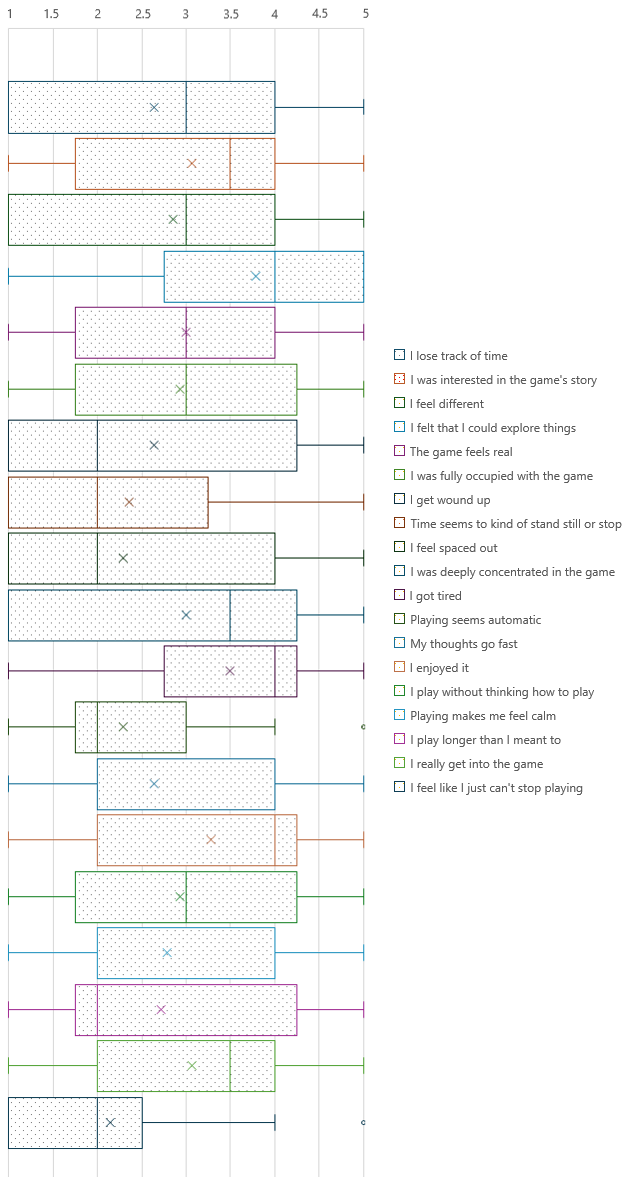
\includegraphics[width=0.8\textwidth]{formA2.png}
    \caption{Wykresy pudełkowe pytań kwestionariusza dla wersji z AI formularza A}
    \label{fig:appendixB_formA2}
\end{figure}

\begin{table}[h!]
    \begin{center}
        \begin{tabular}{|m{10em}|r|r|r|}
            \hline
            Pytanie                                                           & Średnia ocena & Mediana & Odchylenie st. \\
            \hline
            1. Tracę poczucie czasu                                           & 3,7           & 4       & 1,26           \\
            2. Byłem/-am \newline zainteresowany/-a fabułą gry                & 3,8           & 4       & 1,15           \\
            3. Czuję się inaczej                                              & 3,15          & 3       & 1,5            \\
            4. Czułem/-am, że mogę odkrywać różne rzeczy                      & 2,1           & 1       & 1,52           \\
            5. Gra wydaje się prawdziwa                                       & 3,1           & 3,5     & 1,33           \\
            6. Byłem/-am \newline w pełni zajęty/-a grą                       & 3,65          & 4       & 1,39           \\
            7. Denerwuję się                                                  & 2,75          & 3       & 1,55           \\
            8. Czas jakby stanął w miejscu lub się zatrzymał                  & 3,2           & 4       & 1,44           \\
            9. Czuję się \newline rozkojarzony/-a                             & 3,2           & 3       & 1,28           \\
            10. Byłem/-am głęboko \newline skoncentrowany/-a \newline na grze & 3,6           & 3       & 1,27           \\
            11. Zmęczyłem/-am się                                             & 3,2           & 3       & 1,28           \\
            12. Granie wydaje się automatyczne                                & 3,2           & 3       & 1,44           \\
            13. Moje myśli \newline biegną szybko                             & 3,5           & 4       & 1,43           \\
            14. Podobało mi się                                               & 3,95          & 4       & 0,89           \\
            15. Gram bez zastanawiania się jak grać                           & 3,4           & 3,5     & 1,27           \\
            16. Granie sprawia, \newline że czuję się spokojny/-a             & 3,8           & 4       & 0,95           \\
            17. Gram dłużej \newline niż zamierzałem/-am                      & 3,75          & 4       & 1,25           \\
            18. Naprawdę wczuwam się w grę                                    & 3,65          & 4       & 1,27           \\
            19. Czuję, że nie mogę przestać grać                              & 3,15          & 3       & 1,5            \\
            \hline
        \end{tabular}
    \end{center}
    \caption{Statystyki opisowe pytań kwestionariusza dla wersji z AI formularza B}\label{tab1:appendixB_7}
\end{table}

\begin{figure}[h!]
    \centering
    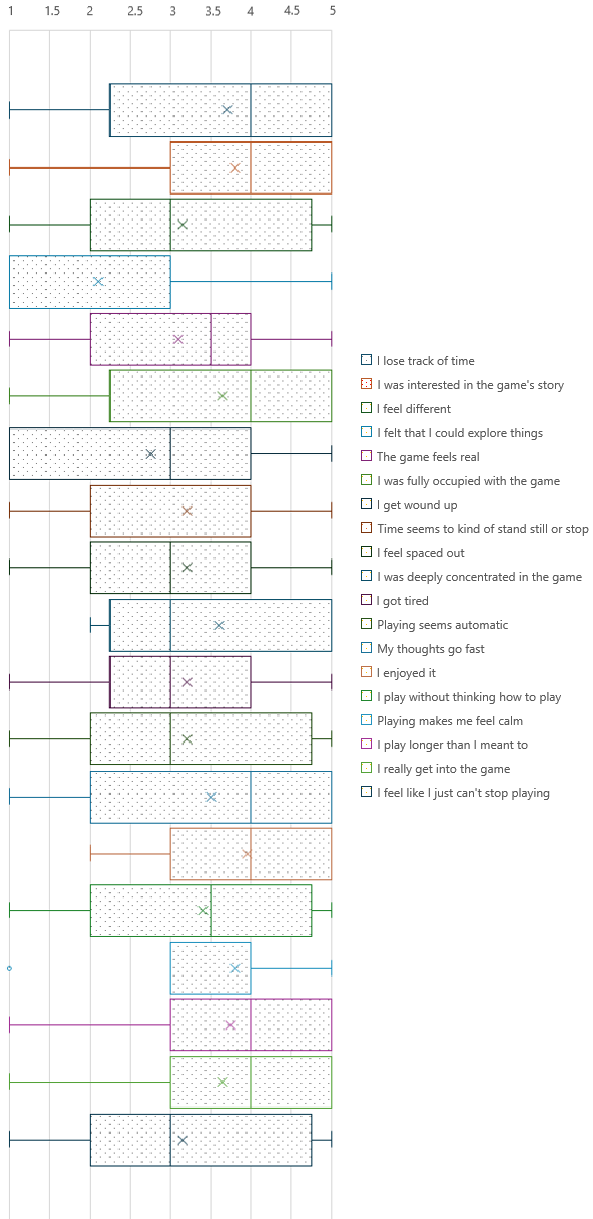
\includegraphics[width=0.75\textwidth]{formB1.png}
    \caption{Wykresy pudełkowe pytań kwestionariusza dla wersji z AI formularza B}
    \label{fig:appendixB_formB1}
\end{figure}

\begin{table}[h!]
    \begin{center}
        \begin{tabular}{|m{10em}|r|r|r|}
            \hline
            Pytanie                                                           & Średnia ocena & Mediana & Odchylenie st. \\
            \hline
            1. Tracę poczucie czasu                                           & 3,1           & 3       & 1,45           \\
            2. Byłem/-am \newline zainteresowany/-a fabułą gry                & 3,5           & 4       & 1,32           \\
            3. Czuję się inaczej                                              & 2,95          & 3       & 1,76           \\
            4. Czułem/-am, że mogę odkrywać różne rzeczy                      & 3,4           & 3,5     & 1,47           \\
            5. Gra wydaje się prawdziwa                                       & 3,25          & 3       & 1,41           \\
            6. Byłem/-am \newline w pełni zajęty/-a grą                       & 3,5           & 4       & 1,47           \\
            7. Denerwuję się                                                  & 2,3           & 2       & 1,53           \\
            8. Czas jakby stanął w miejscu lub się zatrzymał                  & 2,9           & 3       & 1,62           \\
            9. Czuję się \newline rozkojarzony/-a                             & 2,9           & 3       & 1,55           \\
            10. Byłem/-am głęboko \newline skoncentrowany/-a \newline na grze & 3,5           & 4       & 1,36           \\
            11. Zmęczyłem/-am się                                             & 3,4           & 3,5     & 1,50           \\
            12. Granie wydaje się automatyczne                                & 4,15          & 4,5     & 0,99           \\
            13. Moje myśli \newline biegną szybko                             & 3,35          & 4       & 1,42           \\
            14. Podobało mi się                                               & 3,65          & 4       & 1,18           \\
            15. Gram bez zastanawiania się jak grać                           & 4,35          & 4,5     & 0,81           \\
            16. Granie sprawia, \newline że czuję się spokojny/-a             & 3,7           & 3,5     & 1,17           \\
            17. Gram dłużej \newline niż zamierzałem/-am                      & 2,95          & 3       & 1,64           \\
            18. Naprawdę wczuwam się w grę                                    & 3,4           & 3,5     & 1,43           \\
            19. Czuję, że nie mogę przestać grać                              & 3             & 3       & 1,59           \\
            \hline
        \end{tabular}
    \end{center}
    \caption{Statystyki opisowe pytań kwestionariusza dla wersji bez AI formularza B}\label{tab1:appendixB_9}
\end{table}

\begin{figure}[h!]
    \centering
    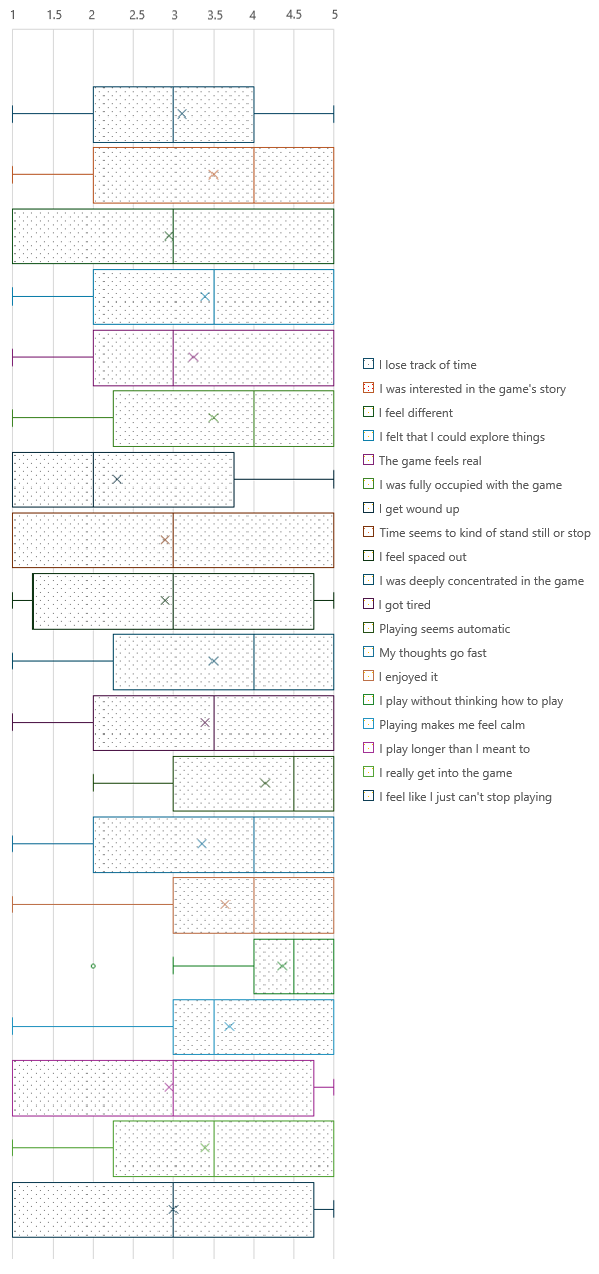
\includegraphics[width=0.74\textwidth]{formB2.png}
    \caption{Wykresy pudełkowe pytań kwestionariusza dla wersji bez AI formularza B}
    \label{fig:ch7_formB2}
\end{figure}